
\section{Serveur marchand}

Pour la partie marchande de l'application, nous avons tout d'abord dû créer le serveur qui s'occuperait de
stocker les données relatives aux produits à vendre, aux commandes, aux caddies, etc.

La première étape a donc été de créer la base de données de ce serveur. Nous avons donc réfléchi à un
ORM (Object-Relational Mapping) qui permettrait de faire le lien entre notre futur serveur, écrit en Java,
et notre base de données, et, après beaucoup de réflexion, nous avons choisi d'utiliser Jooq.

\begin{figure}[H]
    \centering
    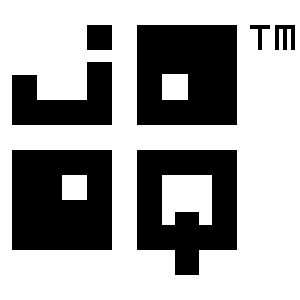
\includegraphics[scale=.2]{./img/joey-jooq-logo.png}
    \caption{Logo de Jooq}
    \label{fig:jooq-logo}
\end{figure}

Jooq est donc un ORM utilisant une approche database-first, ce qui signifie que la base de données doit
d'abord être créée avant de pouvoir l'utiliser. La puissance de cet outil réside dans le fait qu'il permet de
générer automatiquement les classes qui nous permettront d'accéder à notre base de données et à
effectuer des opérations dessus.

La base de données, elle, sera donc créée grâce à JDBC tout simplement. Elle utilisera PostgreSQL, et la
représentation de ses tables :

\begin{figure}[H]
    \centering
    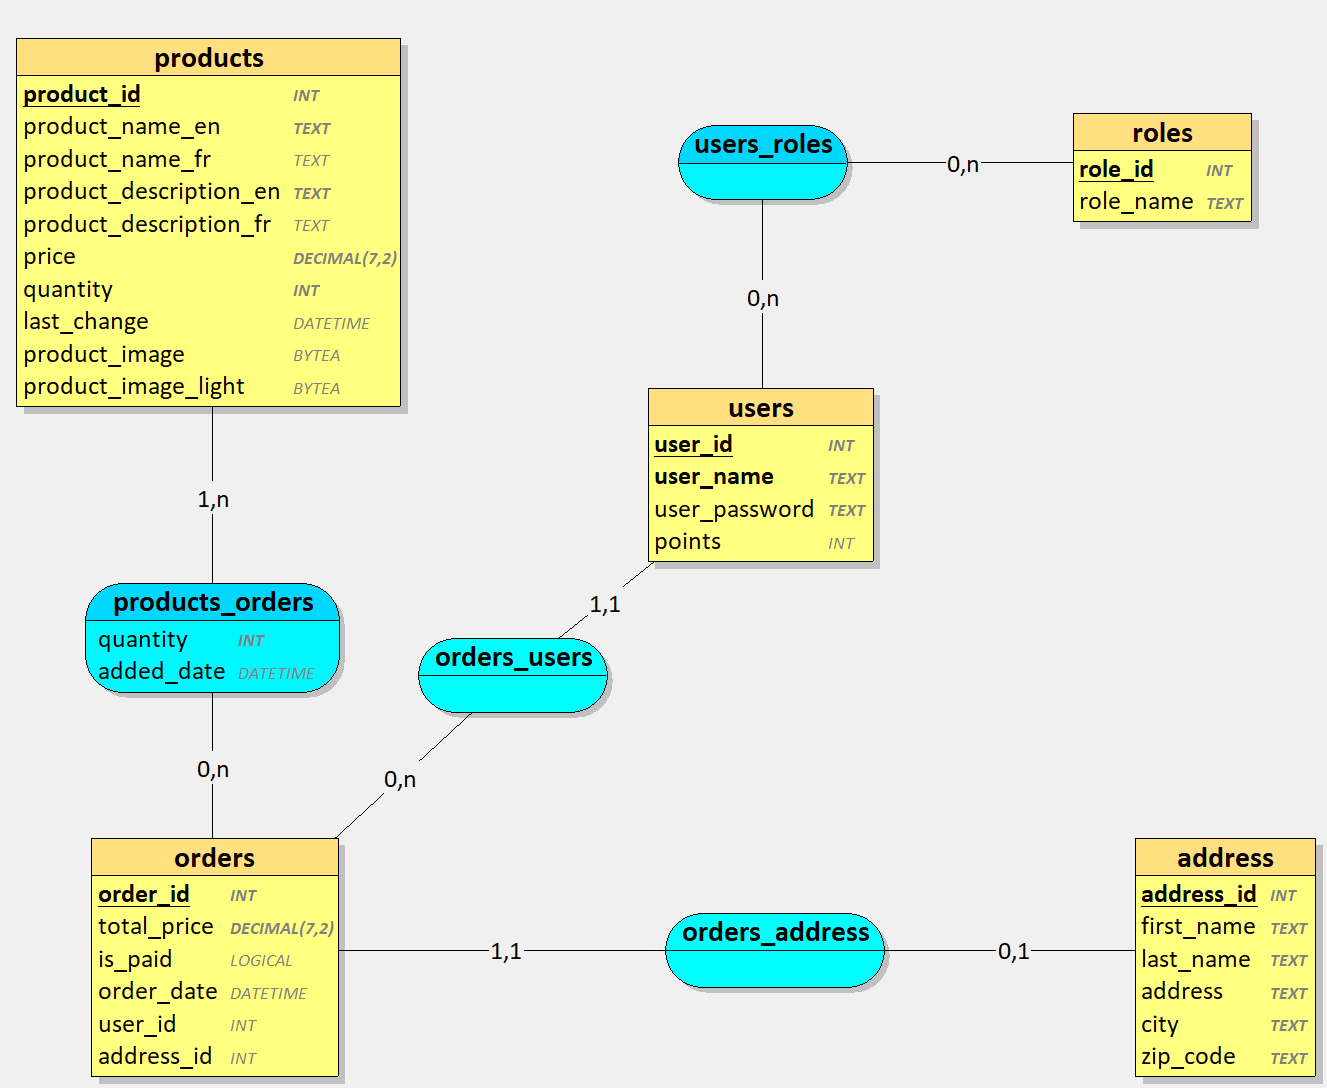
\includegraphics[width=\textwidth]{./img/joey-looping.png}
    \caption{Schéma de la base de données}
    \label{fig:poc-db-looping}
\end{figure}

A noter qu'il n'y a pas de notion de caddie, car c'est le champ \mintinline{java}|is_paid| de la table orders qui permets de savoir si une commande est dans le caddie ou si elle est déjà payée.

Il a ensuite fallu créer l'API qui permettra à l'application Android et au site web marchand d'accéder aux
données. Pour cela, nous avons utilisé Spring Boot, qui est un outil très pratique et puissant, nous
permettant de faire énormément de choses en Java.

\begin{figure}[H]
    \centering
    
\includegraphics[scale=.2]{./img/joey-spring-framework.png}
    \caption{Logo de Spring}
    \label{fig:poc-spring-logo}
\end{figure}

La dernière étape était de sécuriser cette API, accessible en HTTPS, fut d'ajouter un filtre permettant de
n'autoriser que certains utilisateurs à accéder à certains endpoints de l'API. Pour cela, nous avons coupler
Spring Boot à une librairie appelée JWT.io. Cette librairie permet d'implémenter facilement le principe
des JWT (JSON Web Tokens) à notre serveur. Voici leur fonctionnement:

\begin{figure}[H]
    \centering
    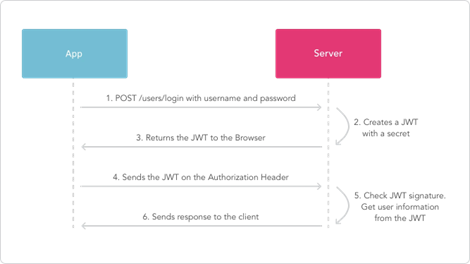
\includegraphics[width=\textwidth]{./img/joey-img-1.png}
    \caption{Échange avec un token JWT}
    \label{fig:poc-jwt-exchange}
\end{figure}

L'utilisateur va, via l'application cliente, s'identifier avec son nom d'utilisateur et son mot de passe. Ces
informations seront envoyées au serveur via une requête HTTP POST.

Le serveur, en recevant ces informations, va tout d'abord identifier l'utilisateur. Une fois cela fait, il va le
JWT, qui est une chaîne de caractère aléatoire générée à partir des informations de l'utilisateur. D'autres
informations seront associées à ces tokens, comme un temps avant expiration par exemple.

Une fois ce token généré, il le renverra au client. Celui-ci le stockera, et pour ses prochaines requêtes, il
mettra ce token dans le champ « Authorization » du header des requêtes. Cela permettra au serveur de
vérifier quel utilisateur envoie la requête, en regardant celui associé au token. Enfin, si l'utilisateur
possède le rôle nécessaire pour accéder au endpoint voulu, le serveur lui enverra la réponse appropriée.

Dans ce serveur, nous aurons 3 rôles possibles pour les utilisateurs:

\begin{itemize}
    \item ROLE\_ADMIN: rôle associé aux administrateurs, donnant accès à tous les endpoints
    \item ROLE\_USER: rôle associé aux utilisateurs lambda de notre application. Ce seront les utilisateurs qui pourront acheter des produits, accéder à leurs caddies, etc.
    \item ROLE\_CARD: rôle utilisé pour pouvoir ajouter et supprimer des points sur les cartes à points des utilisateurs.
\end{itemize}

Le serveur sera divisé en 3 applications distinctes : DatabaseCreation, DatabaseInserts et ApiApplication.

L'application DatabaseCreation permet de générer la base de données grâce à JDBC et les classes utiles à
notre programme grâce à Jooq. Pour configurer ce dernier, il suffit de créer un fichier XML donnant la
configuration de l'outil. Il faut lui donner l'URL de la base de données, le nom d'utilisateur, le mot de
passe, ainsi que d'autres paramètres relatifs à la génération des classes.

L'application DatabaseInserts permet d'insérer les valeurs de base de notre base de données, ainsi que
les différents produits vendus par notre application. Les données à insérer se trouvent dans un fichier
CSV, ce qui permet de pouvoir modifier facilement les valeurs que l'on veut insérer. Voici un exemple
d'insertion utilisant Jooq:

\begin{listing}[H]
    \begin{minted}{java}
UserRecord user1 = context.newRecord(users.USERS);
user1.setUserName("user1");
user1.setUserPassword(bCryptPasswordEncoder.encode("password_user1"));
user1.store();
    \end{minted}
    \caption{Définition des variables et des fonctions présentes sur la Java Card}
    \label{listing:creation-user1}
\end{listing}

Parmi ces valeurs se trouvent les champs product\_image et product\_image\_light. La différence entre ces
2 champs est que le premier est plus volumineux que le second. Le premier sera envoyé lorsque l'on veut
accéder à la description d'un produit en particulier, tandis que le second, lui, sera envoyé lorsque l'on
demande à accéder à la liste des produits, afin de réduire la bande passante utilisée ainsi que les temps
de chargement. Il existe également des champs de nom et de description en anglais et en français, afin
de contribuer à l'internationalisation de notre application.

ApiApplication est simplement l'API. Implémentée grâce à Spring Boot, elle possède plusieurs endpoints
utiles à tous les utilisateurs. A noter que, par manque de temps, les JWT utilisés pour l'API n'auront pas
de date d'expiration.

La sécurisation des endpoints est assurée grâce à un Bean créé avec Spring Boot, qui permet de préciser qui a accès à quoi:

\begin{listing}[H]
    \begin{minted}{java}
@Bean
public SecurityFilterChain filterChain(HttpSecurity http) throws Exception {
    http
            .httpBasic().disable()
            .csrf().disable()
            .sessionManagement().sessionCreationPolicy(SessionCreationPolicy.STATELESS)
            .and()
            .authorizeHttpRequests()
            .requestMatchers("/auth/signin").permitAll()
            .requestMatchers("/auth/signup").permitAll()
            .requestMatchers(HttpMethod.GET, "/products/**").permitAll()
            .requestMatchers(HttpMethod.POST, "/products/**").hasAuthority("ROLE_ADMIN")
            .requestMatchers(HttpMethod.GET, "/users/orders").hasAnyAuthority("ROLE_USER", "ROLE_ADMIN")
            .requestMatchers(HttpMethod.GET, "/users/cart").hasAnyAuthority("ROLE_USER", "ROLE_ADMIN")
            .requestMatchers(HttpMethod.GET, "/users/**").hasAnyAuthority("ROLE_ADMIN", "ROLE_CARD")
            .requestMatchers(HttpMethod.POST, "/users/**").hasAnyAuthority("ROLE_ADMIN", "ROLE_CARD")
            .requestMatchers(HttpMethod.GET, "/orders/*/products").hasAnyAuthority("ROLE_USER", "ROLE_ADMIN")
            .requestMatchers(HttpMethod.GET, "/orders/payment").permitAll()
            .requestMatchers(HttpMethod.GET, "/orders/**").hasAuthority("ROLE_ADMIN")
            .requestMatchers(HttpMethod.POST, "/orders/add").hasAnyAuthority("ROLE_USER", "ROLE_ADMIN")
            .requestMatchers(HttpMethod.POST, "/orders/remove").hasAnyAuthority("ROLE_USER", "ROLE_ADMIN")
            .requestMatchers(HttpMethod.POST, "/orders/*/validate").hasAnyAuthority("ROLE_USER", "ROLE_ADMIN")
            .requestMatchers(HttpMethod.POST, "/orders/**").hasAuthority("ROLE_ADMIN")
            .anyRequest().authenticated()
            .and()
            .apply(new JwtConfigurer(jwtTokenProvider));

    return http.build();
}
    \end{minted}
    \caption{Définition des variables et des fonctions présentes sur la Java Card}
    \label{listing:joey-filter-chain}
\end{listing}

Un thread est également créé afin de supprimer les objets des caddies des utilisateurs lorsqu'ils ont été
ajoutés il y a trop longtemps, afin de faire de la place. Ce thread se réveille à intervalle régulier pour
effectuer cette opération.

\section{Android}

Notre application Android est composée de 2 activités : une pour la connexion, et une pour le magasin en
ligne. En effet, il est conseillé d'utiliser le moins d'activités possibles, car les passages de données et les
transitions sont plus simples et optimisées par fragments.
Nous avons utilisé l'API 28, compatible avec Android 9.0 (Pie).

Au début pensée pour être faite en Java, nous avons décidé de faire notre application en Kotlin
principalement grâce aux coroutines, un moyen d'effectuer des tâches asynchrones, ce qui est plus léger
que les Thread du Java et qui sont donc plus adaptées aux applications mobile, celles-ci devant être le
plus léger possible.

Tout d'abord, voici l'écran de connexion :

\begin{figure}[H]
    \centering
    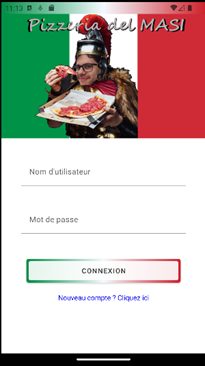
\includegraphics[scale=.9]{./img/joey-img-4.png}
    \caption{Écran de connexion de l'application mobile}
    \label{fig:poc-login-screen}
\end{figure}

Cette page toute simple prend seulement le nom d'utilisateur et le
mot de passe afin de pouvoir se connecter. Nous pouvons cliquer sur
le texte tout en-dessous pour créer un nouveau compte si nous le voulons.

Si un compte a déjà été ajouté, une page permettant de de
sélectionner un des comptes ajoutés sur le téléphone se mettra à la place de celle-ci.

L'enregistrement des utilisateurs est géré par l'AccountManager d'Android. C'est une solution simple et
sécurisée de mémoriser un utilisateur ainsi que le token d'authentification qui leur est associé sur
n'importe quel téléphone Android.

Pour le mettre en place, il faut tout d'abord créer une classe étendant la classe abstraite
AbstractAccountAuthenticator. Cette classe contient 2 méthodes notables à overrider : addAccount et
getAuthToken.

Dans addAccount, il faut créer un Intent emmenant l'utilisateur à la page de connexion ou d'ajout de
compte. Il faut qu'à la fermeture de l'activité, le compte soit ajouté à l'appareil. Les comptes ajoutés
peuvent être vus dans la section « Comptes et mots de passe » des paramètres du téléphone:

\begin{figure}[H]
    \centering
    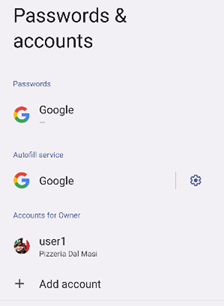
\includegraphics[scale=.9]{./img/joey-img-5.png}
    \caption{AccountManager d'Android}
    \label{fig:poc-account-manager}
\end{figure}

La deuxième méthode, getAuthToken, récupère le token associé à un utilisateur et, s'il n'existe pas,
ramène l'utilisateur vers la page de connexion.

La deuxième étape est de créer un service, ce qui permettra d'ajouter les utilisateurs grâce à la page
montrée ci-dessus. Voici le code de ce service, assez simple:

\begin{listing}[H]
    \begin{minted}{kotlin}
class CustomAuthenticatorService: Service() {
    override fun onBind(p0: Intent?): IBinder? {
        val customAccountAuthenticator = CustomAccountAuthenticator(this)
        return customAccountAuthenticator.iBinder
    }
}
    \end{minted}
    \caption{}
    \label{listing:bind-thing}
\end{listing}

Une fois connecté, l'utilisateur arrivera sur la page des produits que nous vendons :

\begin{figure}[H]
    \centering
    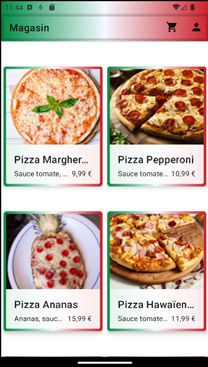
\includegraphics[scale=.9]{./img/joey-img-6.png}
    \caption{Liste des produits de l'application mobile}
    \label{fig:poc-pizzas}
\end{figure}

Cette liste est créée grâce à une RecyclerView, qui décharge les objets de la liste qui ne sont plus visibles sur l'écran, bien que toujours accessibles, ce qui améliore les performances de
l'application.

Cette liste est une liste « infinie », c'est-à-dire que l'utilisateur peut scroller sans s'arrêter. Une fois qu'il a atteint la fin de la liste, de nouveaux objets sont chargés et placés à la suite de la liste actuelle, ce qui permet de ne pas charger la liste entière de tous les produits d'un coup. Pour obtenir ce comportement, il suffit d'implémenter un listener de scroll, qui chargera de nouveaux objets quand la fin de la liste est atteinte.

En cliquant sur l'un des produits, l'utilisateur accèdera à sa page de description et pourra l'ajouter à son caddie s'il le souhaite.

Dans les paramètres de l'utilisateur, seules 3 options sont disponibles : Déconnexion, historique de commandes et langues.

L'historique de commandes affiche simplement les commandes passées, avec leur date et le prix total payé. En cliquant sur l'une des commandes, on peut y voir ses détails :

\begin{figure}[H]
    \centering
    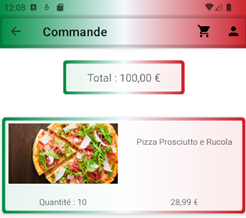
\includegraphics[scale=.9]{./img/joey-img-7.png}
    \caption{Aperçu d'une commande}
    \label{fig:poc-commande}
\end{figure}

Le bouton langue permet de changer la langue choisie par l'utilisateur. Par défaut, l'application utilise la
langue par défaut du téléphone. Mais cette page permet de changer cette langue :

\begin{figure}[H]
    \centering
    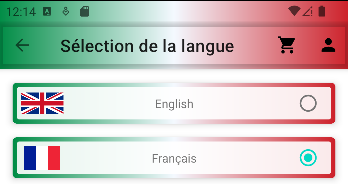
\includegraphics[width=\textwidth]{./img/joey-img-8.png}
    \caption{Liste des produits de l'application mobile}
    \label{fig:poc-lang}
\end{figure}

L'information quant à la préférence de langue d'un utilisateur sera sauvegardée dans une base de
données Room.

Enfin, nous avons la page du caddie. Elle est très similaire à la page des produits de l'historique des
commandes, à la différence qu'ici, il y a un bouton pour passer la commande.

Lors du passage de commande, il faut que l'utilisateur entre l'adresse de destination. Cette adresse sera
envoyée au serveur marchand afin de verrouiller la commande. Une fois cela fait, l'utilisateur accèdera à
au portail de paiement web.

Lorsque le paiement sera effectué, le client enverra le token de paiement généré au serveur marchand,
qui vérifiera l'existence de ce token. S'il existe bien, le paiement sera validé et le champ is\_paid de la
commande dans la base de données sera mis à true.

La base de données, implémentée grâce à Room, ne comporte qu'une seule table, celle des utilisateurs,
ne permettant de stocker que les préférences de ceux-ci. Ce choix a été fait car nous avons jugé que
stocker des transactions localement lorsqu'il n'y a plus de connexion pour les effectuer automatiquement
lors de la prochaine connexion pourrait causer des problèmes de sécurité. De plus, nous ne connaissons
aucune autre application implémentant de genre de comportement. Nous pensions stocker le caddie
localement, mais des problèmes similaires auraient pu survenir. C'est pourquoi nous avons choisi de ne
stocker que les préférences dans la base de données.

Voici le fonctionnement d'une base de données Room :

\begin{figure}[H]
    \centering
    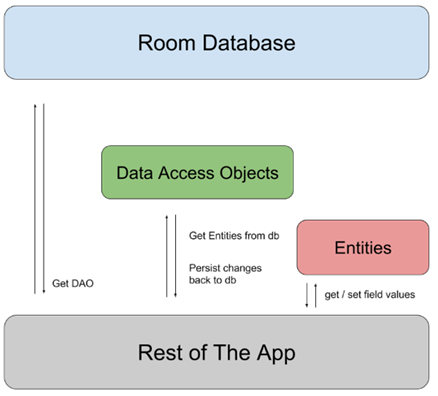
\includegraphics[width=\textwidth]{./img/joey-img-9.png}
    \caption{Fonctionnement d'une base de donnée Room}
    \label{fig:poc-room}
\end{figure}

Les données seront insérées et récupérées de la base de données via des DAO, qui contiennent des
méthodes permettant d'effectuer ces opérations. Ces DAO sont implémentés grâce à des interfaces.
Les données récupérées seront simplement stockées dans des classes de données, les entités.

\section{National bank server (NBS)}

Le NBS est une passerelle entre les banques et les bases de données destinées aux data scientists. Son
principe est tel qu'il faut que les banques puissent envoyer les données des authentifications et des
transactions détectées aux bases de données via ce NBS, et donc, nous avons logiquement fait du NBS
une API. Son fonctionnement est exactement le même que le serveur marchand. Les seules différences
résident dans les tables stockées, les endpoints ainsi que les rôles et utilisateurs associés.
Ici, nous avons simplement 2 rôles possibles :

\begin{itemize}
    \item ROLE\_ADMIN : Pour les administrateurs. Permet d'accéder à tous les endpoints.
    \item ROLE\_BANK : Ce rôle permet aux banques d'envoyer leurs données. Elles n'auront accès qu'aux méthodes permettant d'effectuer ces actions.
\end{itemize}

